\begin{salyga}
Stačiakampio $ABCD$ kraštinių ilgiai yra $AB=8\,\text{cm}$ ir
$BC=6\,\text{cm}$. Įstrižainės $AC$ ir $BD$ susikerta taške $O$.
\begin{center}
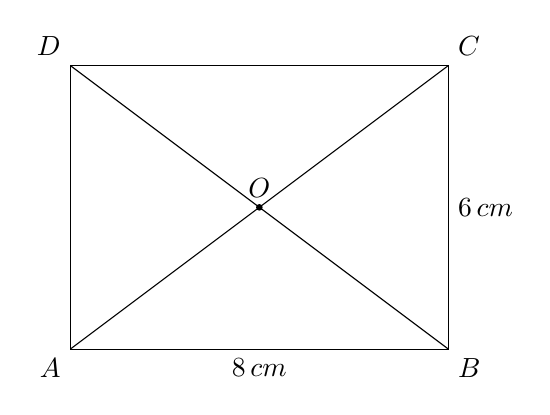
\begin{tikzpicture}[scale=0.6]
  \coordinate (A) at (0,0);
  \coordinate (B) at (8,0);
  \coordinate (C) at (8,6);
  \coordinate (D) at (0,6);
  \coordinate (O) at (4,3);
  \draw (A)--node[below] {$8\,\text{cm}$}(B)
    --node[right] {$6\,\text{cm}$}(C)--(D)--cycle;
  \draw (A)--(C) (B)--(D);
  \fill (O) circle (2pt);
  \node[below left] at (A) {$A$};
  \node[below right] at (B) {$B$};
  \node[above right] at (C) {$C$};
  \node[above left] at (D) {$D$};
  \node[above] at (O) {$O$};
\end{tikzpicture}
\end{center}
\begin{enumerate}[label=\alph*)]
  \item Apskaičiuokite įstrižainės $AC$ ilgį.
  \item Įrodykite, kad $AO=BO=CO=DO$, ir raskite šių atkarpų ilgį.
  \item Apskaičiuokite trikampio $AOB$ plotą.
\end{enumerate}
\end{salyga}

\begin{atsakymas}
\begin{enumerate}[label=\alph*)]
  \item $AC=10\,\text{cm}$.
  \item $AO=BO=CO=DO=5\,\text{cm}$.
  \item $S_{AOB}=12\,\text{cm}^2$.
\end{enumerate}
\end{atsakymas}

\begin{sprendimas}
\begin{enumerate}[label=\alph*)]
\item Kadangi $\angle ABC=90^\circ$, pagal Pitagoro teoremą
\[
  AC=\sqrt{AB^2+BC^2}=\sqrt{8^2+6^2}=10\,\text{cm}.
\]
Trikampis $BAD$ taip pat statusis, o $AD=BC=6\,\text{cm}$, todėl
$BD=\sqrt{AB^2+AD^2}=10\,\text{cm}$.

\item Įrodysime, kad įstrižainės dalija viena kitą pusiau.
Kadangi $AB\parallel CD$, tai $\angle BAO=\angle DCO$ ir
$\angle ABO=\angle CDO$ (vidaus priešiniai kampai).
Be to, $AB=CD$, nes tai priešingos stačiakampio kraštinės.
Taigi trikampiai $ABO$ ir $CDO$ yra lygūs pagal kraštinę ir du
kampus prie jos. Vadinasi, $AO=CO$ ir $BO=DO$.
Kadangi $AC=BD=10\,\text{cm}$, gauname
\[
  AO=CO=\frac{AC}{2}=5\,\text{cm},\qquad
  BO=DO=\frac{BD}{2}=5\,\text{cm}.
\]

\item Nuleiskime iš $O$ statmenį $OH$ į kraštinę $AB$.
Trikampiai $AHO$ ir $ABC$ panašūs: jų kampai ties $H$ ir $B$
statūs, o kampas ties $A$ bendras, nes $H\in AB$ ir $O\in AC$.
Todėl
\[
  \frac{OH}{BC}=\frac{AO}{AC}=\frac12,
  \qquad OH=3\,\text{cm}.
\]
Trikampio plotas lygus pusei pagrindo ir aukštinės sandaugos:
\[
  S_{AOB}=\frac12\,AB\cdot OH
  =\frac12\cdot8\cdot3=12\,\text{cm}^2.
\]
\end{enumerate}
\hfill$\square$
\end{sprendimas}
